\documentclass{template/socthesis}

\usepackage{subcaption} 
\usepackage{amsmath} 
\usepackage{enumitem} 
\usepackage{hyperref} % reference
\usepackage{gensymb} % balíček symbolů
\usepackage{booktabs}

\usepackage[toc,page]{appendix}
\usepackage{color} % balíček pro obarvování textů
\usepackage{xcolor}  % zapne možnost používání barev, mj. pro \definecolor
\definecolor{mygreen}{RGB}{0,150,0} % nastavení barev odkazů 
\usepackage{listings} % balíček pro formátování zdrojových kódů 
\usepackage[author=,status=final]{fixme} % vkládání poznámek  
% dva módy (status): draft (poznámky se zobrazují v PDF) / final (poznámky se nezobrazují v PDF)
\usepackage{multirow}

\lstset { %
    language=C++,
    backgroundcolor=\color{black!5}, % set backgroundcolor
    basicstyle=\footnotesize,% basic font setting
}

\addbibresource{text.bib} % soubor s bibliografií
\nocite{*}

\titlecz{Automatický skleník} % český název práce
\titleen{Automatic greenhouse} % anglický název práce
\author{Petr Štourač} % jméno a příjmení autora
\field{7} % obor (pouze číslo, zbytek vysází šablona - číslo oboru viz http://www.soc.cz/obory-soc/)
\school{Střední průmyslová škola a~Vyšší odborná škola Brno, Sokolská, příspěvková organizace} % celý název školy
\mentor{Mgr. Miroslav Burda} % jméno a příjmení školitele
\mentorstatement{Mgr. Miroslava Burdy} % jméno a příjmení ve druhém pádě 

% Změňte, pokud se liší
%\region{Jihomoravský} % kraj
\placefooter{Brno 2020} % místo a rok

% hinty k používání balíčků hyperref, url, hyperlink a hypertarget
% \usepackage{hyperref} % balíček pro hypertextové odkazy
% \url{www.odkaz.cz}
% \href{http://www.odkaz.cz}{Text který bude jako odkaz}
% \hyperlink{label}{proklikávací_text} - odkaz na text 
% \hypertarget{label}{cíl_odkazu} - cíl odkazu 

\begin{document} % konec preambule dokumentu

\maketitle % vysází titulky

\makecopyrightstatement{V~Brně} % místo

% poděkování
\makethanks{Děkuji svému školiteli Mgr. Miroslavu Burdovi za obětavou pomoc, podnětné připomínky a~hlavně nekonečnou trpělivost, kterou mi během práce poskytoval.}

\pagestyle{empty}

\section*{Anotace}
\color{mygreen}
Anotace má za úkol stručně popsat cíle práce a velmi stručný úvod k tématu. 
Většinou bývá použit první odstavec úvodu.
\color{black}

Zahradničení je dnes naprosto běžnou zájmovou činností. Mnoho lidí mající takovou zálibu je ovšem velmi časově vytížených. Kromě práce se musí starat mnohdy i o~rodinu a~na péči o~rostliny jim často jednoduše nezbývá čas. Jedním z~těchto lidí je i můj táta, který mě inspiroval k~vytvoření PROTOPlantu -- systému pro snadnou a~levnou automatizaci skleníku. 

Cílem práce je vytvořit univerzální a~dostupný systém pro automatizaci skleníku, který by usnadnil péči o~rostliny časově vytíženým lidem. 

\subsection*{Klíčová slova}
\color{mygreen}
Klíčová slova.
Snažte se najít alespoň 5, ideálně i více klíčových slov, která jednoduše vystihují vaši práci.
\color{black}

automatizace skleníku, ESP32, PROTOPlant, automatizace, open-source hardware, open-source software

\newpage % pokud se práce vleze na jednu stránku, tento rádek zakomentuj

\vspace{20mm}

\section*{Annotation}
\color{mygreen}
Zde přijde anglický překlad anotace.
\color{black}

Gardening is a~very common hobby today. However, many people who likes this activity doesn't have enough time for it. 
Beside work, they have to take care of their families and after this, they don't have any time to take care of plants. 
My dad is exactly this kind of man. 
And that inspired me to create PROTOPlant -- system for easy and cheap greenhouse automation.

Goal of this thesis is to create universal and available system for greenhouse automation, that will make it easier for these people to take care of their plants.

\subsection*{Keywords}
\color{mygreen}
Klíčová slova - jejich překlad do angličtiny.
\color{black}

greenhouse automation, ESP32, PROTOPlant, automation, open-source hardware, open-source software

\newpage
\pagestyle{plain}

\tableofcontents % vysází obsah

%%% Začátek práce
\setcounter{figure}{0}
\setcounter{table}{0}
\newpage

% zde můžeš s pomocí příkazu \input{cesta k souboru} vložit soubory; doporučuji každou větší kapitolu dát do samostatného souboru pro větší přehlednost

% Úvod práce
\chapter*{Úvod}
\addcontentsline{toc}{chapter}{Úvod}
Pěstování skleníkových rostlin je dnes naprosto běžnou zájmovou činností. 
Ať již člověk pěstuje zeleninu, orchideje, nebo technické plodiny, vždy dojde k~závěru, že na ně mnohdy nemá čas.
Když přijde domů z~práce, musí se postarat o~rodinu, připadně dodělat jiné činnosti a~na rostliny již jednoduše čas nezbývá.
Jedním z~těchto lidí je i můj táta.
Velmi rád pěstuje orchideje, které má ve skleníku.
Ovšem postupem času na ně má z~pracovních důvodů stále méně a~méně času.
Proto mne napadlo, že lidí, kteří na tom jsou tak, jako on je jistě mnoho.
To mne inspirovalo k~vytvoření PROTOPlantu -- systému pro levnou a~snadnou automatizaci skleníku dostupného každému. 

Cílem této práce je vytvořit univerzální a~dostupný systém pro automatizaci skleníku, který by usnadnil péči o~rostliny časově vytíženým lidem. 

Systémy pro takovouto automatizaci dnes existují, jsou ovšem určeny primárně pro velkozemědělství, nikoli pro člověka, který ve skleníku pěstuje několik druhů zeleniny pro sebe, aby ji nemusel kupovat v~obchodě, nebo který vlastní menší skleník s~okrasnými rostlinami. 

Samozřejmě, na internetu existuje spousta návodů, jak si nějaký takový „systém“ vyrobit za pomoci Arduina, nepájivého pole a~\uv{pár} drátků.
Takové řešení se mi ovšem nezdá příliš univerzální a~pracující lidé nemají mnohdy čas si takto hrát.
Zároveň pro sestavení něčeho takovového potřebují mít určité znalosti v~elektrotechnice a~programování.

Kromě toho jsem chtěl, aby bylo možno systém v~budoucnu připojit k~internetu a~sledovat jej tak například z~dovolené.
\newline

Při vytváření práce jsem si dal za cíl, aby byl systém:
\begin{itemize}
    \item kompletně open-source
    \item levný
    \item modulární
    \item snadný na ovládání
    \item univerzální
\end{itemize}

Dalším z~cílů tohoto projektu je úspora energií (elektřina, voda), které lze díky automatizaci dosáhnout.

\newpage


% Motivace
\chapter{Kapitola}
Lorem ipsum dolor sit amet, consectetur adipiscing elit.
Aliquam nunc magna, sollicitudin id leo eu, viverra congue risus.
Aliquam consequat ipsum ut erat placerat consequat nec at diam. 
Aenean est odio, molestie sit amet nunc in, pretium luctus elit. 
Donec imperdiet orci vel porttitor placerat. 
Proin ut hendrerit elit, ultricies accumsan urna. 
Vivamus condimentum lorem viverra lectus finibus, nec volutpat turpis auctor.
Cras quis felis non lorem consectetur interdum eu eu sem. 
Proin sit amet feugiat metus. 
Ut vitae orci a enim vestibulum porta. 

\section{Oddíl}
Lorem ipsum dolor sit amet, consectetur adipiscing elit.
Aliquam nunc magna, sollicitudin id leo eu, viverra congue risus.
Aliquam consequat ipsum ut erat placerat consequat nec at diam. 
Aenean est odio, molestie sit amet nunc in, pretium luctus elit. 
Donec imperdiet orci vel porttitor placerat. 
Proin ut hendrerit elit, ultricies accumsan urna. 
Vivamus condimentum lorem viverra lectus finibus, nec volutpat turpis auctor.
Cras quis felis non lorem consectetur interdum eu eu sem. 
Proin sit amet feugiat metus. 
Ut vitae orci a enim vestibulum porta. 

\subsection{Pododdíl}
Lorem ipsum dolor sit amet, consectetur adipiscing elit.
Aliquam nunc magna, sollicitudin id leo eu, viverra congue risus.
Aliquam consequat ipsum ut erat placerat consequat nec at diam. 
Aenean est odio, molestie sit amet nunc in, pretium luctus elit. 
Donec imperdiet orci vel porttitor placerat. 
Proin ut hendrerit elit, ultricies accumsan urna. 
Vivamus condimentum lorem viverra lectus finibus, nec volutpat turpis auctor.
Cras quis felis non lorem consectetur interdum eu eu sem. 
Proin sit amet feugiat metus. 
Ut vitae orci a enim vestibulum porta. 

\paragraph{Odstavec}
Lorem ipsum dolor sit amet, consectetur adipiscing elit.
Aliquam nunc magna, sollicitudin id leo eu, viverra congue risus.
Aliquam consequat ipsum ut erat placerat consequat nec at diam. 
Aenean est odio, molestie sit amet nunc in, pretium luctus elit. 
Donec imperdiet orci vel porttitor placerat. 
Proin ut hendrerit elit, ultricies accumsan urna. 
Vivamus condimentum lorem viverra lectus finibus, nec volutpat turpis auctor.
Cras quis felis non lorem consectetur interdum eu eu sem. 
Proin sit amet feugiat metus. 
Ut vitae orci a enim vestibulum porta. 

\subparagraph{Pododstavec}
Lorem ipsum dolor sit amet, consectetur adipiscing elit.
Aliquam nunc magna, sollicitudin id leo eu, viverra congue risus.
Aliquam consequat ipsum ut erat placerat consequat nec at diam. 
Aenean est odio, molestie sit amet nunc in, pretium luctus elit. 
Donec imperdiet orci vel porttitor placerat. 
Proin ut hendrerit elit, ultricies accumsan urna. 
Vivamus condimentum lorem viverra lectus finibus, nec volutpat turpis auctor.
Cras quis felis non lorem consectetur interdum eu eu sem. 
Proin sit amet feugiat metus. 
Ut vitae orci a enim vestibulum porta. 

\newpage

% Konkurence
\chapter{Kapitola 2}
Lorem ipsum dolor sit amet, consectetur adipiscing elit.
Aliquam nunc magna, sollicitudin id leo eu, viverra congue risus.
Aliquam consequat ipsum ut erat placerat consequat nec at diam. 
Aenean est odio, molestie sit amet nunc in, pretium luctus elit. 
Donec imperdiet orci vel porttitor placerat. 
Proin ut hendrerit elit, ultricies accumsan urna. 
Vivamus condimentum lorem viverra lectus finibus, nec volutpat turpis auctor.
Cras quis felis non lorem consectetur interdum eu eu sem. 
Proin sit amet feugiat metus. 
Ut vitae orci a enim vestibulum porta:
\begin{itemize} % odrážkový seznam
    \item lorem
    \item ipsum
    \item lorem ipsum
    \item lipsum
\end{itemize}

\begin{table}[h]
    \centering
    \resizebox{\textwidth}{!}{%
    \begin{tabular}{@{}l|lll@{}}
        & \textbf{Průmyslová řešení} & \textbf{„Kutilská“ řešení} & \textbf{PROTOPlant}                                                                                   \\ \midrule
    \textbf{Dodání}      & Výroba na zakázku          & „Vyrob si sám“             & \begin{tabular}[c]{@{}l@{}}Možnost sestavení přímo doma, \\ nebo dodání \B{hotového} systému\end{tabular} \\
    \textbf{Cena}        & Drahá ($>$~10~000~Kč)      & Levná ($<$~10~000~Kč)      & Kompromis cena -- výkon (již od 2~500~Kč)                                                                               \\
    \textbf{Ovládání}    & Komplexní                  & Jednoduché (většinou)      & Jednoduché                                                                                            \\
    \textbf{Konektivita} & Většinou ethernet          & Často Wi-Fi                & \begin{tabular}[c]{@{}l@{}}Wi-Fi, Bluetooth, \\ možnost přidání podpory Ethernetu\end{tabular}        \\
    \textbf{Řízení}      & PLC                        & Většinou Arduino           & ESP32                                                                                                 \\ \bottomrule
    \textbf{Modularita}  & Ano                        & Ne                         & Ano                                                                                                   \\
    \textbf{Univerzálnost}& Ano                       & Ne                         & Ano                                                                                                   \\ 
    \textbf{Open-source} & Ne                         & Většinou ano               & Ano                                                                                                   \\ \bottomrule    
    \end{tabular}%
    }
    \caption{Tabulka srovnání PROTOPlantu a~jiných řešení.}
    \label{tab:COMPARATION}
\end{table}

\begin{figure}[htbp]
    \centering
    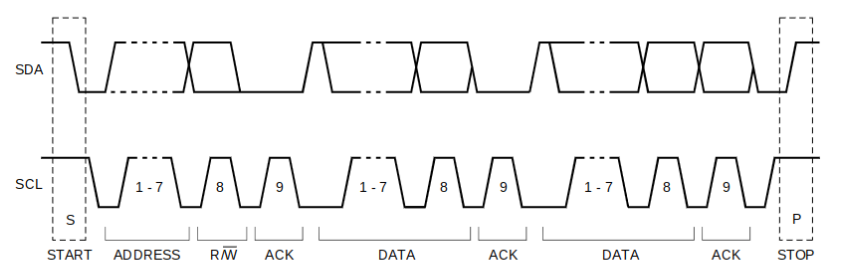
\includegraphics[width=\textwidth]{img/I2C.png}
    \caption{Celý datový přenos po I2C sběrnici. Převzato z~\cite{I2C_specs}}
    \label{fig:I2C-protocol}
 \end{figure}
 
\noindent\B{Lipsum} -- lorem ipsum dolor sit amet, consectetur adipiscing elit.
Aliquam nunc magna, sollicitudin id leo eu, viverra congue risus.
Aliquam consequat ipsum ut erat placerat consequat nec at diam. 
Aenean est odio, molestie sit amet nunc in, pretium luctus elit. 
Donec imperdiet orci vel porttitor placerat. 
Proin ut hendrerit elit, ultricies accumsan urna. 
Vivamus condimentum lorem viverra lectus finibus, nec volutpat turpis auctor.
Cras quis felis non lorem consectetur interdum eu eu sem. 
Proin sit amet feugiat metus. 
Ut vitae orci a enim vestibulum porta. \newline

\section{Sumarizace}
Nabídka řešení v~tomto oboru je velmi chudá.
Na jedné straně stojí průmyslová řešení, která jsou drahá a~dodávají se primárně do skleníků velkých zemědělských firem.
Na opačném břehu jsou řešení amatérská. 
Ta jsou ovšem buďto naprosto nepoužitelná v~běžně velkém skleníku (primárně je uživatelé vyrábí pro malá pařeniště), nebo neuniverzální.

\newpage

% Zaver prace
\chapter*{Závěr}
\addcontentsline{toc}{chapter}{Závěr}
Záměrem mojí práce bylo vytvořit univerzální systém pro automatizaci skle\-ní\-ku, který je:
\begin{itemize}
    \item open-source
    \item levný
    \item modulární
    \item snadný na ovládání
    \item univerzální
\end{itemize}

Tento cíl se mi podařilo splnit.
Lidé, kteří mají zájem si systém vytvořit najdou veškerou dokumentaci, schémata a~zdrojový kód na webu \textit{\url{www.protoplant.cz}}.

Díky SOČ jsem se naučil pracovat se softwarem pro návrh PCB Autodesk EAGLE.
Zároveň jsem vylepšil své schopnosti v~programování a~získal spoustu dalších zkušeností v~elektrotechnice a~s~prací na takto komplexních projektech.

Část svých plánů do budoucna jsem již nastínil v~kapitole \ref{sec:DISTRIBUTION}.
PROTOPlant plánuji začít vyrábět průmyslově a~prodávat jej.
Zároveň jej budu dále vylepšovat a~přidávat další funkce.
V~bližší době plánuji dokončit všechny právě rozpracované moduly a~začít implementovat funkci pro vzdálený přístup a~sledování přes internet (například z~práce, nebo z~dovolené).
Dále bych pro PROTOPlant vyvinul vlastní mobilní aplikaci, která uživateli umožní snadno a~rychle vzdáleně sledovat stav skleníku, měnit nastavení, nebo jej ovládat.

Momentálně běží PROTOPlant v~jednom skleníku. 
Toto číslo bych během následujícího roku rád alespoň zdvacetinásobil. 

\newpage
\newpage

\appendix
\addcontentsline{toc}{chapter}{Přílohy}
% Tistene spoje a elektronika
\chapter{Elektronika a~tištěné spoje}
Všechny prototypy základních desek PROTOPlantu byly založeny na univerzálních tištěných spojích. Vzhledem k~tomu, že jsem po stránce vzhledu i funkčnosti nebyl s~takovýmto provedením spokojen, rozhodl jsem se nechat vyrobit vlastní tištěné spoje pro základní desku i senzorové moduly.
Díky tomuto jsem se naučil návrhu tištěných spojů a~tvorbě výrobních podkladů v~programu Autodesk EAGLE.

\section{PPMB32 -- Základní deska}
\label{subsec:motherBoard}
Základní deska je rozdělena do několika částí. 
Vzhledem k~tomu, že umím pájet velmi dobře, rozhodl jsem se pro ruční osazení všech součástek, které byly doposud osazeny pouze na různých modulech připojených k~základní desce, včetně procesoru ESP32-WROOM32D.
Z~důvodu přehlednosti jsem desku rozdělil do několika částí:

\begin{itemize}
    \item Control (ESP32-WROOM32D a~programátor)
    \item H-power (napájecí obvod a~H-můstky)
    \item SIN (SensorIN -- piny pro připojení senzorů)
    \item POUT (PowerOUT -- výstup pro napájení dalších periferií)
    \item PanCon (PanelConnect -- piny pro připojení tlačítek a~displeje na ovládacím panelu)
    \item SelfProt (SelfProtection -- senzor teploty a~piny pro připojení vnitřního detektoru vody)
\end{itemize} 

Samotná základní deska má dvě verze. Jejich rozdíly jsou vysvětleny níže.
Obě verze desky jsou kromě sekce Control osazeny stejným hardwarem, tedy:

\begin{itemize}
    \item 2x H-můstek VNH2SP30
    \item regulátory napětí 7805CV-DG od STMicroelectronics
    \item pinheady pro připojení senzorů, ovládacího panelu a~dalších periferií
    \item svorkovnicemi pro připojení napájecích kabelů a~silových výstupů
\end{itemize}

Kromě dalších součástek je přímo na desce osazen senzor DS18B20 chránící desku před přehřátím. 
Pokud teplota základní desky překročí 50~\degree C, automaticky se přeruší veškeré operace a~systém přejde do režimu nouzového chlazení (viz kapitola \ref{paragraph:CoolingMode}).

\paragraph{PPMB32-F}
Kompletní, samostatná deska. 
Je přímo osazena procesorem ESP32-WROOM32D i programátorem CP2102N. 
Má nižší profil, tudíž je možné ji použít i v~menších prostorech.
Integrovaný programátor lze s~pomocí jumperů odpojit a~přes programovací piny připojit externí. Tuto verzi jsem nazval PPMB32-F (označení F od anglického slova Full -- kompletní).
Zároveň je optimalizovaná pro strojní osazování.

\paragraph{PPMB32-E}
Vzhledem k~tomu, že je PROTOPlant veřejně dostupný, nebyl jsem si jist, zda by kompletní osazení takto velké desky zvládl i laik. 
Napadlo mě proto vytvořit i druhou desku, na které by byly osazeny dutinkové lišty pro vsazení vývojové ESP32 DevKitC. 
Odpadla by tedy nutnost kompletně osazovat sekci Control. 
Tuto verzi jsem nazval PPMB32-E (označení E od anglického slova Easy -- jednoduchý).
Je určena primárně pro ruční osazování.

\paragraph{Sekce Control}
Jak již bylo zmíněno, tato část desky zahrnuje modul procesoru ESP32-WROOM32D a~programovací obvod. 
Ten se skládá z~převod\-ní\-ku USB-UART CP2102N, tranzistorů SS8050-G (sloužících pro reset procesoru), indikačních LED diod a~mikro USB konektoru. 
Nachází se zde i jumper pro přepínání mezi externím programátorem a~programátorem přímo na desce.

\paragraph{Sekce H-power}
V~této části desky se nacházejí H-můstky VNH2SP30 společně s~regulátory napětí 7805CV-DG (výstup 5VDC) a~LM3940IT-3.3 (výstup 3,3VDC). 
Na verzi PPMB32-F je dále osazen AMS1117-3.3 pro napájení procesoru. 

V~dolní části desky se poté nacházejí dva integrované obvody VNH2SP30, z~nichž jeden (VNH1) je určen pro ovládání aktuátorů manipulujících s~okny a~druhý 
(VNH2) má několik režimů funkce podle připojeného výstupu:
\begin{itemize}
    \item disabled (výstupy jsou deaktivovány)
    \item pump (VNH je použito pro spínání čerpadla, případně stykače řídícího čerpadlo)
    \item heating (VNH je použito pro řízení topné spirály)
\end{itemize}

Napájení desky je rozděleno do tří okruhů. 

\paragraph{Okruh A}
\label{par:PowerCircuitA}
Tento okruh je určen pro napájení řídící elektroniky.
Má celkově 3 části, oddělené s~pomocí stabilizátorů napětí.
Jejich propojení znázorňuje schéma.
Rozsah vstupního napětí pro tento okruh je 7,5~VDC až 18~VDC.

\paragraph{Okruhy V1 a~V2}
Použity pro oddělené napájení jednotlivých výstupů. 
Jejich napájecí rozsahy jsou rozepsány v~tabulce \ref{fig:powerSourceCharsVNH}.

\begin{table}[h]
    \centering
    \begin{tabular}{llll}
        \hline
        \multicolumn{1}{|l|}{\textbf{Parametr}}           & \multicolumn{1}{l|}{\textbf{Min.}} & \multicolumn{1}{l|}{\textbf{Max.}} & \multicolumn{1}{l|}{\textbf{Jednotka}} \\ \hline
        \multicolumn{1}{|l|}{Vstupní napětí}              & \multicolumn{1}{l|}{5,5}           & \multicolumn{1}{l|}{16}            & \multicolumn{1}{l|}{V}                 \\ \hline
        \multicolumn{1}{|l|}{Výstupní napětí}             & \multicolumn{1}{c|}{-}             & \multicolumn{1}{l|}{16}            & \multicolumn{1}{l|}{V}                 \\ \hline
        \multicolumn{1}{|l|}{Výstupní proud}              & \multicolumn{1}{c|}{-}             & \multicolumn{1}{l|}{30}            & \multicolumn{1}{l|}{A}                 \\ \hline
        \multicolumn{1}{|l|}{Maximální kontinuální proud} & \multicolumn{1}{c|}{-}             & \multicolumn{1}{l|}{14}            & \multicolumn{1}{l|}{A}                 \\ \hline
    \end{tabular}
    \caption{Tabulka napájecích rozsahů napájecích větví VNH1 a~VNH2}
    \label{fig:powerSourceCharsVNH}
\end{table}

\paragraph{Sekce SIN}
Sekce s~piny pro připojení jednotlivých senzorů. 
S~výjimkou ochranných rezistorů je složena pouze z~pinheadů.
Jednotlivé piny jsou pro lepší přehlednost označeny přímo na desce a~podrobněji popsány v~jejím datasheetu (viz kapitola \ref{sec:DPS_datasheets}). 

\paragraph{Sekce POUT} 
Piny pro připojení napájení dalších periferií, modulů, či senzorů.
Je připojena k~napájecímu okruhu A.
Piny jsou rozděleny na části připojené k~subokruhům A1 a~A2 s~napětím 3,3 a~5~VDC.

\paragraph{Sekce PanCon}
Dvanáctipinový konektor PanCon slouží pro připojení kabelu od hlavního řídícího panelu. 
Samotný konektor má dva zemnící vývody, dva napájecí (1~x~5~V~a~1~x~3,3~V), dva vývody sběrnice I\textsuperscript{2}C a~6 vývodů pro připojení tlačítek a~přepínačů.
Přesnější zapojení je opět k~dispozici v~datasheetech jednotlivých desek (viz kapitola \ref{sec:DPS_datasheets}).

\section{PPSB -- Desky se senzory teploty a~vlhkosti}
Desky osazené senzory DS18B20\cite{DS18B20} (PPSB-T) a~DHT22\cite{DHT22} (PPSB-TH).
Pro oba typy desek jsem navrhl a~s~pomocí 3D tisku vyrobil vlastní krabičky viz příloha \ref{fig:PPSB-T_cases}.\newline

\noindent\B{PPSB-T} -- deska osazená jedním senzorem DS18B20 \cite{DS18B20} zapojeným v~režimu parazitního napájení (viz \autoref{sec:DS18B20}).
V~něm je senzor napájen přímo ze sběrnice OneWire, stačí mu tedy pro připojení pouze dva kabely (více v~\cite{DS18B20}).
Deska má jednu vstupní a~jednu výstupní stranu, senzory se takto dají řetězit.

Vizualizaci desky naleznete na obrázku \ref{fig:PPSB-T_VISUAL}.\newline \newline

\begin{figure}[h]
    \centering
   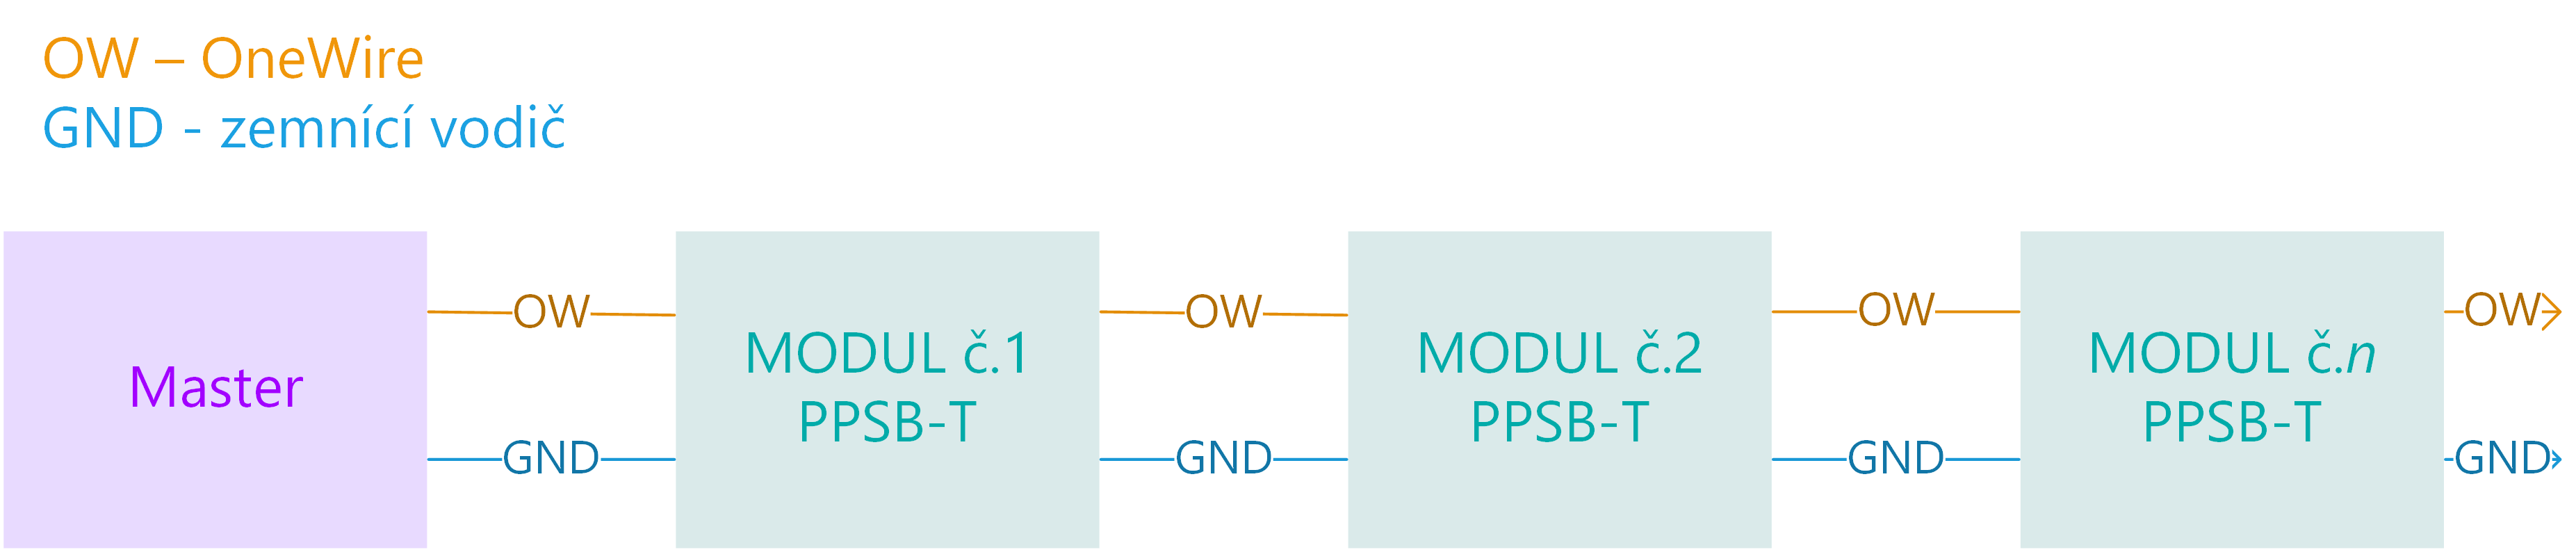
\includegraphics[width=\textwidth]{img/HARDWARE/PPSB-T_CHAIN.png}
   \caption{Řetězení desek PPSB-T.}
   \label{fig:PPSB-T_wiring}
\end{figure}

\noindent\B{PPSB-TH} osazena senzorem DHT22 \cite{DHT22} je schopna měřit vzdušnou vlhkost i teplotu.
Více o~tomto senzoru naleznete v~kapitole \ref{sec:DHT22}.
Narozdíl od PPSB-T tyto desky nelze řetězit.
Vizualizace naleznete na obrázku \ref{fig:PPSB-TH_VISUAL}.\newline

\section{Datasheety DPS PROTOPlantu}
\label{sec:DPS_datasheets}
Další informace k~jednotlivým DPS vytvořeným v~rámci PROTOPlantu budou k~dispozici v~jejích datasheetech, které budou po jejich dokončení (předpokládám 16.~3.~2020) zveřejněny na webu \textit{\url{www.protoplant.cz}}.

\section{Senzorika}
PROTOPlant primárně podporuje 3 typy senzorů. 
DS18B20 pro měření vzdušné teploty, DHT22 schopné měřit vlhkost i teplotu vzduchu a~senzory pro měření vlhkosti půdy.
Dále PROTOPlant podporuje připojení senzorů vlhkosti půdy pracujících na bázi elektrické vodivosti.

\subsection{DS18B20}
\label{sec:DS18B20}
Senzory určené pro měření teploty. 
Komunikují po sběrnici OneWire (více v~\cite{DS18B20}, str. 4) vytvořené společností Maxim Integrated.
Jsou určeny pro teplotní rozsahy -55~\degree C až +125~\degree C.
V~měřícím rozsahu -10~\degree C až +85~\degree C jsou schopny měřit s~přesností na $\pm0,5$~\degree C.
K~PPCU je možno připojit až 30 těchto senzorů.

%\subsection{BME280}
%\label{sec:BME280}
%To be done.

\subsection{Senzory půdní vlhkosti}
\fxnote[author=PŠ]{Dopíšu během pondělka}

\subsection{DHT22}
\label{sec:DHT22}
Čidla, která měří vzdušnou vlhkost i teplotu.
Jejich přesnost je $\pm2\%$ relativní vlhkosti a~$\pm$0,5\degree C.
Opakovatelnost měření je poté $\pm$1\% relativní vlhkosti a~$\pm$0,2\degree C.
Tyto senzory komunikují jednosběrnicově, není tedy možno je řetězit.
K~PPCU je možno připojit těchto senzorů až 6.
Více viz \cite{DHT22}.

Do budoucna zvažuji přechod na senzory AM2321 \cite{AM2321} vzhledem k~tomu, že narozdíl od DHT22 dokáží komunikovat po sběrnici I\superscript{2}C (viz kapitola \ref{sec:I2C_comm}).

\newpage

% Podrobny popis softwaru
\chapter{Software základní desky}
Tato kapitola se zaměřuje na software základní desky PROTOPlantu a~detailně popisuje jeho funkci.
Na software ostatních modulů se zaměřuje následu\-jí\-cí kapitola \ref{chap:moduleSoftware}.

\fxnote[author=PŠ]{\textcolor{mygreen}{Přidat pár ukázek kódu.}}

%\paragraph{Blokové schéma funkce softwaru základní desky}
%Schéma funkce softwaru základní desky je shrnuto blokovým diagramem XXX.

\section{Sdílené knihovny}
Z~důvodu usnadnění programování základní desky i ostatních rozšiřujících modulů jsem vytvořil několik sdílených knihoven. 
V~nich je zahrnuto:
\begin{itemize}
    \item konfigurace systému
    \item nastavení jednotlivých pinů dle standardního rozložení, vč. možnosti nastavení vlastního
    \item práce s~displayem
    \item práce s~tlačítky
    \item řízení H-můstků
    \item ovládání senzorů
\end{itemize}
Díky těmto knihovnám je většina zdrojového kódu uložena v~nich. 
Koncový uživatel, který se rozhodne software modifikovat, poté pouze v~hlavním programu definuje, které moduly spustit a~do konfiguračního souboru zapíše nastavení daných modulů.

\paragraph{Konfigurace softwaru}
Konfigurace softwaru pro jednotlivé verze hardwaru je řešena pomocí jednoho souboru.
Podle toho, jak jsou jednotlivá makra v~tomto souboru definována, prekompilátor následně sestaví software přímo pro danou verzi.
Část konfiguračního souboru je zobrazena níže.
V~této části lze nastavit parametry přístupového bodu Wi-Fi, který si PROTOPlant sám vytvoří, sériové linky a~displeje.
\begin{lstlisting}
    //If wifi credentials not set OR wifi not found, 
    //create own AP with these credentials
    #define AP_SSID ProtoPlant
    #define AP_PASSWORD protoplant
    
    #define SERIAL_DEBUGGING    true
    #define SERIAL_BAUDRATE     115200
    
    #define DISPLAY_CONNECTED   true
    #define DISPLAY_ADDRESS     0x27
    #define DISPLAY_TIMEOUT     10000
    #define DISPLAY_COLONS      16
    #define DISPLAY_ROWS        4
\end{lstlisting}

\section{Datové sběrnice}
PROTOPlant primárně využívá dvě datové sběrnice:
\begin{itemize}
    \item I\superscript{2}C
    \item OneWire
\end{itemize}

\noindent\B{Sběrnici I\superscript{2}C} používá PROTOPlant pro komunikaci se zařízeními na stejné desce, případně pro řízení LCD displeje instalovaného na řídícím panelu (připojení přes PanCon). 
\label{sec:I2C_comm}

\subparagraph{Princip}
Na sběrnici je připojeno jedno zařízení jakožto master (řídící) a~jedno či více zařízení jako slave (řízená).
Tato zařízení jsou navzájem propojena dvěma dráty (proto se I\superscript{2}C někdy přezdívá TwoWire), serial clock (SCL) a~serial data (SDA).
Každé ze slave zařízení má sedmibitovou adresu (např. 0xE0), která musí být pro každé zařízení na jedné sběrnici odlišná.
Některá zařízení mají tuto adresu pevně zapsanou a~nelze ji měnit, zatímco u~jiných ji lze změnit.
Zařízení připojené jako v~režimu master tuto adresu nepotřebuje, vzhledem k~tomu, že on sám vždy adresuje jen jedno ze zařízení.

\subparagraph{Komunikační protokol}
Za klidového stavu (neprobíhá žádná komunikace) jsou obě linky (SDA i SCL) připojeny nastaveny na HIGH.
Jakmile chce master zahájit komunikaci, vyšle takzvaný startovní signál, po kterém následuje adresa daného zařízení, jejíž nultý bit určí, zda chce master číst, nebo zapisovat.
Dále následují datové bity.
Jakmile jsou všechna data přene\-se\-na, vyšle master stop signál, čímž ukončí komunikaci a~sběrnice se vrátí do klidu.
Rychlost celého přenosu určuje pulsování linky CLK.
Celý proces názorně zobrazuje obrázek \ref{fig:I2C-protocol}.

\begin{figure}[htbp]
   \centering
   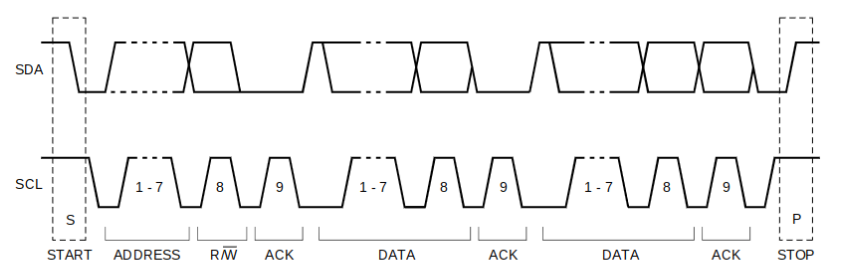
\includegraphics[width=\textwidth]{img/I2C.png}
   \caption{Celý datový přenos po I2C sběrnici. Převzato z~\cite{I2C_specs}}
   \label{fig:I2C-protocol}
\end{figure}

\paragraph{Sběrnice OneWire}
Sběrnici OneWire používá PROTOPlant pro komunikaci s~teplotními čidly DS18B20. 
Více o~této komunikační sběrnici v~\cite{DS18B20}.

\section{Komunikace mezi řídící jednotkou a~jednotlivými moduly}
PROTOPlant podporuje dva režimy komunikace řídící jednotky s~přídavnými moduly:
\begin{itemize}
    \item bezdrátová komunikace přes Wi-Fi
    \item kabelová komunikace přes UART (standard RS-485)
\end{itemize}

\section{Bezdrátová komunikace}
Je vhodná primárně pro malé skleníky v~oblastech, kde nehrozí zarušení signálu.
Tento způsob komunikace je zatím stále ve vývoji.

\section{Kabelová komunikace a~RS-485}
Kabelová komunikace probíhá přes tzv. UART (Universal Asynchronnous Receiver and Transmitter -- univerzální asynchronní přijímač a~vysílač).
PROTO\-Plant využívá průmyslový standard RS-485 umožňující komunikaci s~pomocí dvojlinky.
Opět je zde uplatněn princip master -- slave (řídící jednotka je master, ostatní moduly slave).
Pro tento způsob komunikace existuje několik protokolů, pro příklad velmi často používaný ModBus, nebo nedávno vytvořený JANUS\cite{JANUS}, který používám. 
Více o~principu RS-485 a~samotném protokolu v~\cite[21-25]{JANUS}

\chapter{Software dalších modulů}

\label{chap:moduleSoftware}
Software přídavných modulů je navržen tak, aby k~jeho běhu nebyl zapotřebí velký výpočetní výkon.
Obecně lze jejich funkci znázornit blokovým diagramem \ref{fig:PPCU-to-MODULE-communication}.

\section{Zvláštní stavy}
PROTOPlant má několik zvláštních stavů, ve kterých pracuje v~omezeném režimu.
Tyto stavy slouží primárně pro zabránění poškození systému.

\paragraph{Režim nouzového chlazení}
\label{paragraph:CoolingMode}
Do tohoto režimu přejde systém v~případě, že teplotní senzor na základní desce PPCU detekuje přehřívání. 
Dojde k~automatickému vypnutí výstupů řídící jednotky.
Poté se systém restartuje, aby vyloučil chybu softwaru.
V~případě, že softwarovou chybu nedetekuje, vyčká, než se teplota sníží na běžnou provozní hodnotu, kterou průběžně vypočítává z~průměrů hodnot naměřených před prudkým nárůstem.
Po ochlazení systém pokračuje v~normálním chodu, ovšem na displeji zůstane upozornění, že k~chybě došlo.

\newpage

% Prilohy
\chapter{Obrazové přílohy}

\begin{figure}[h]
    \centering
    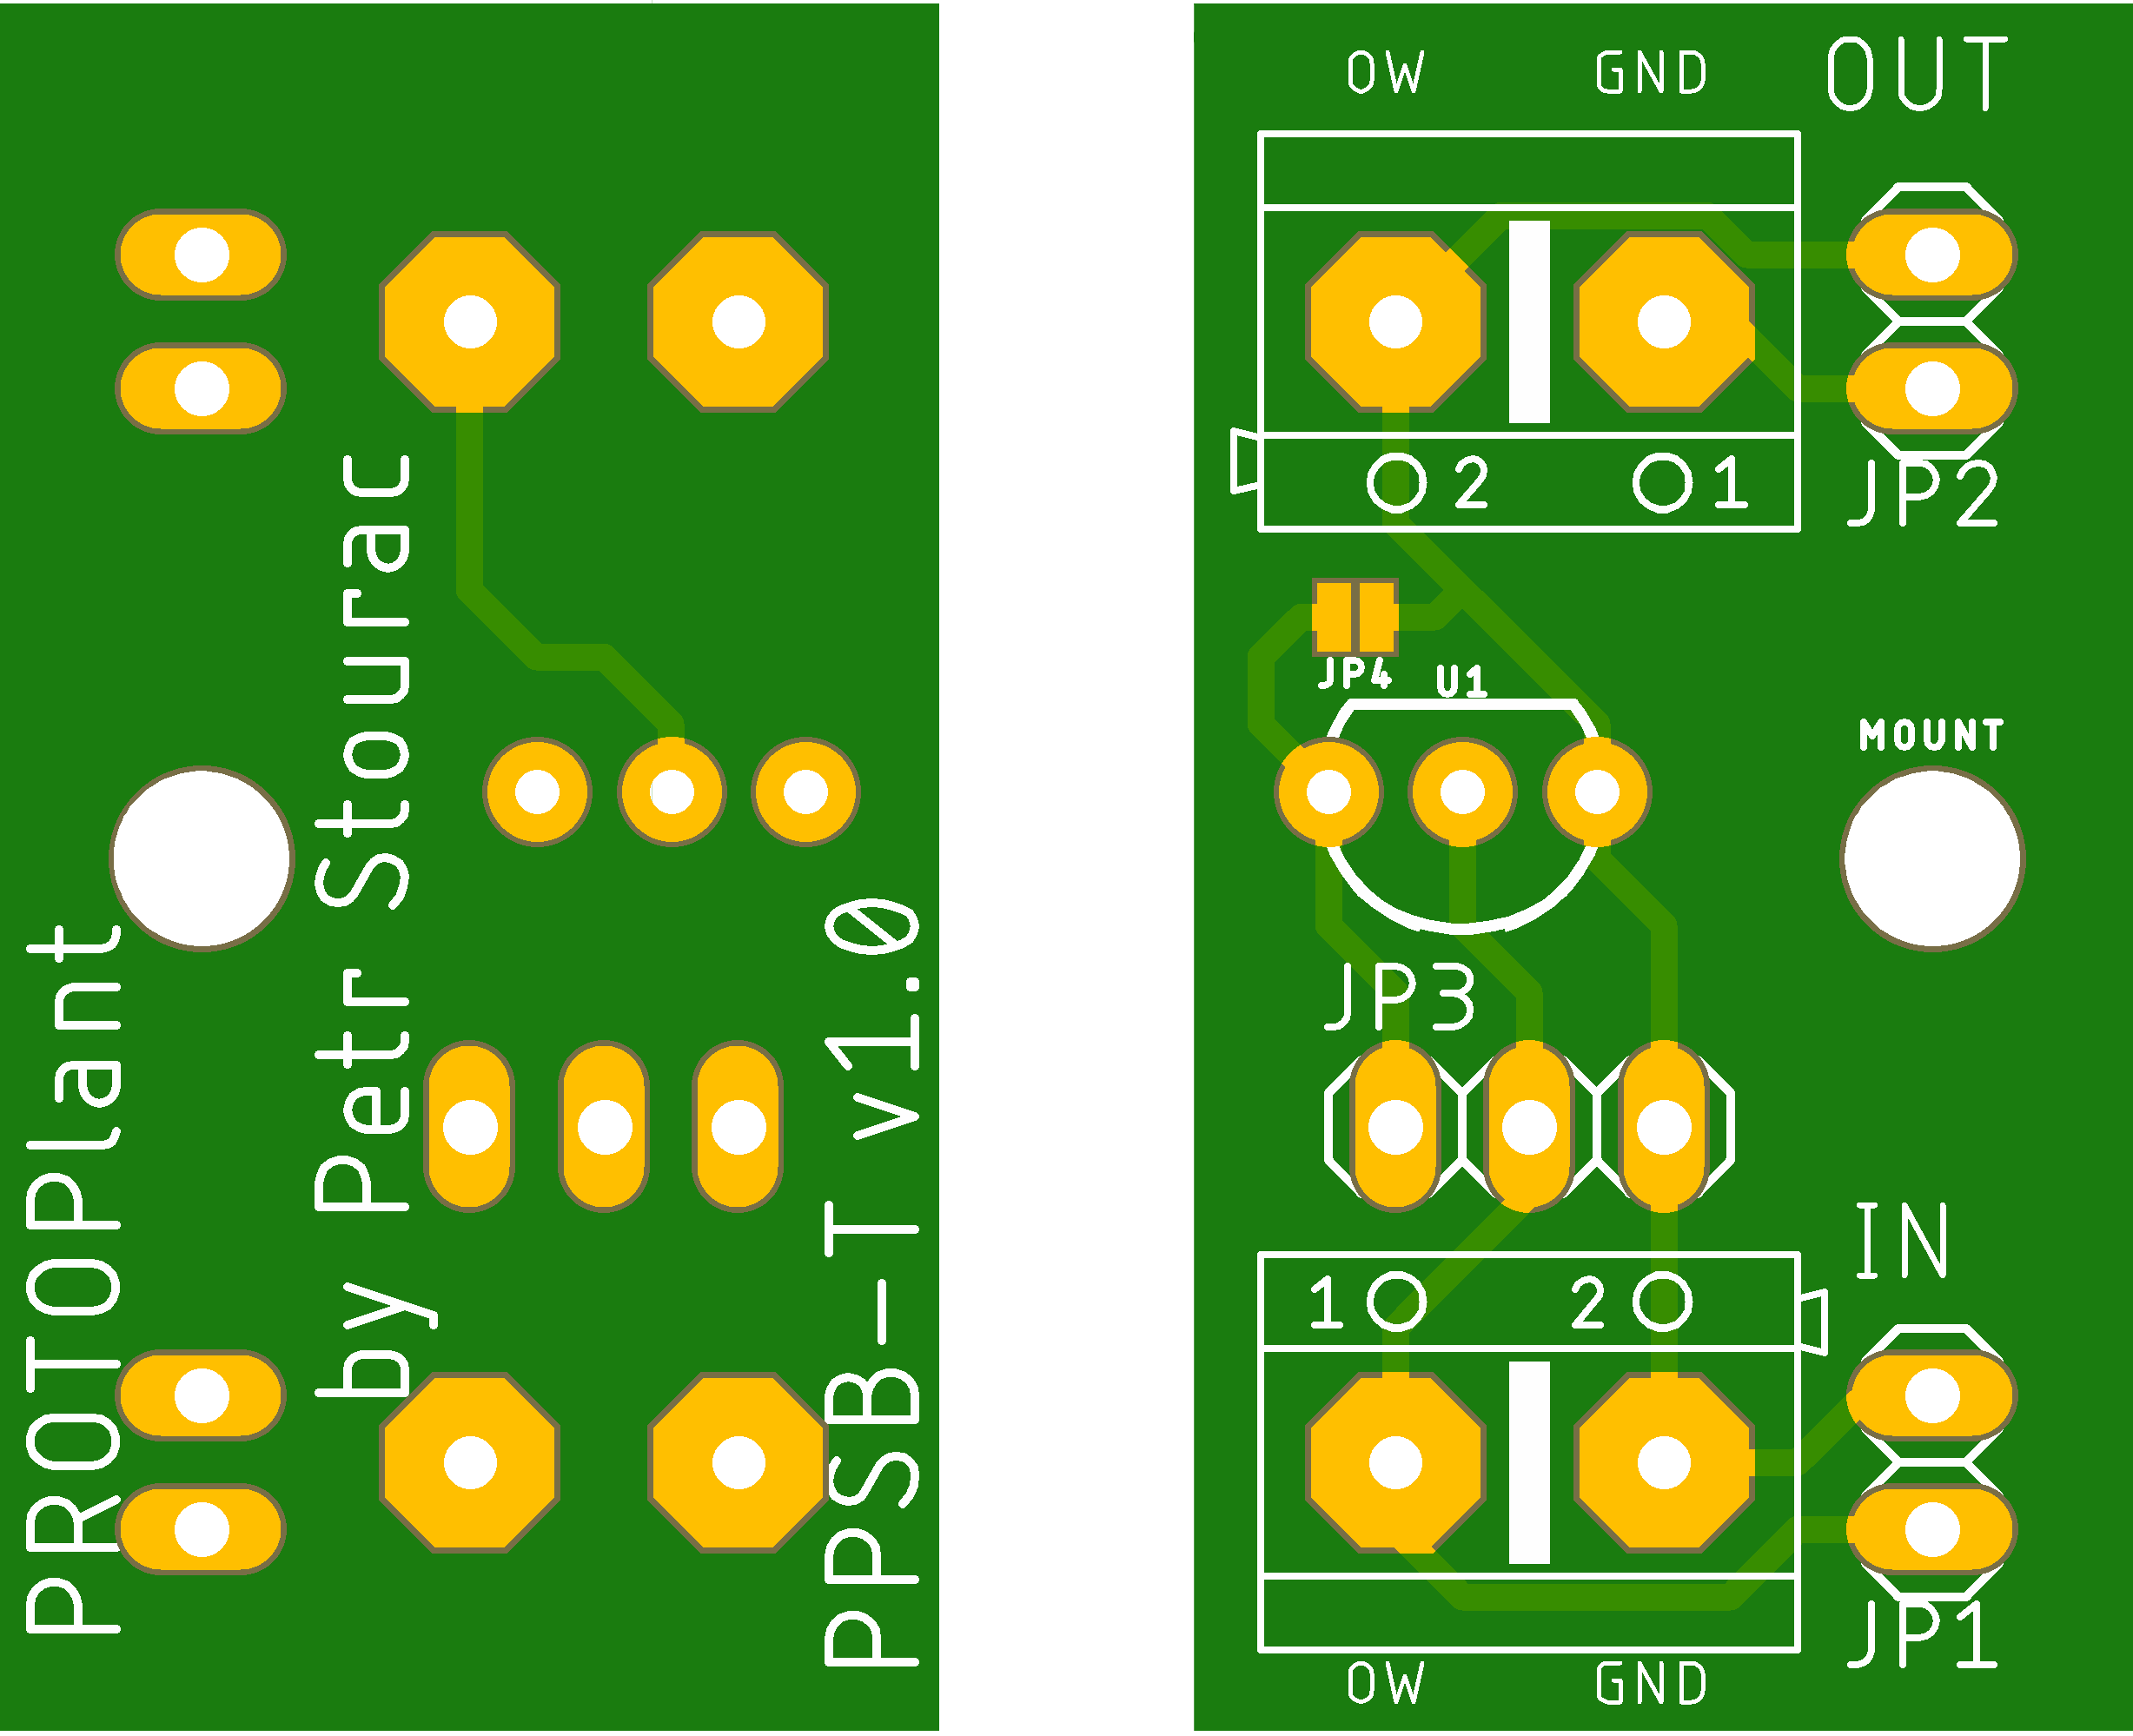
\includegraphics[width=0.85\textwidth]{img/HARDWARE/PPSB-T_BOTH.png}
    \caption{Vizualizace PPSB-T (horní strana vpravo, dolní vlevo).}
    \label{fig:PPSB-T_VISUAL}
\end{figure}

\begin{figure}[h]
    \centering
    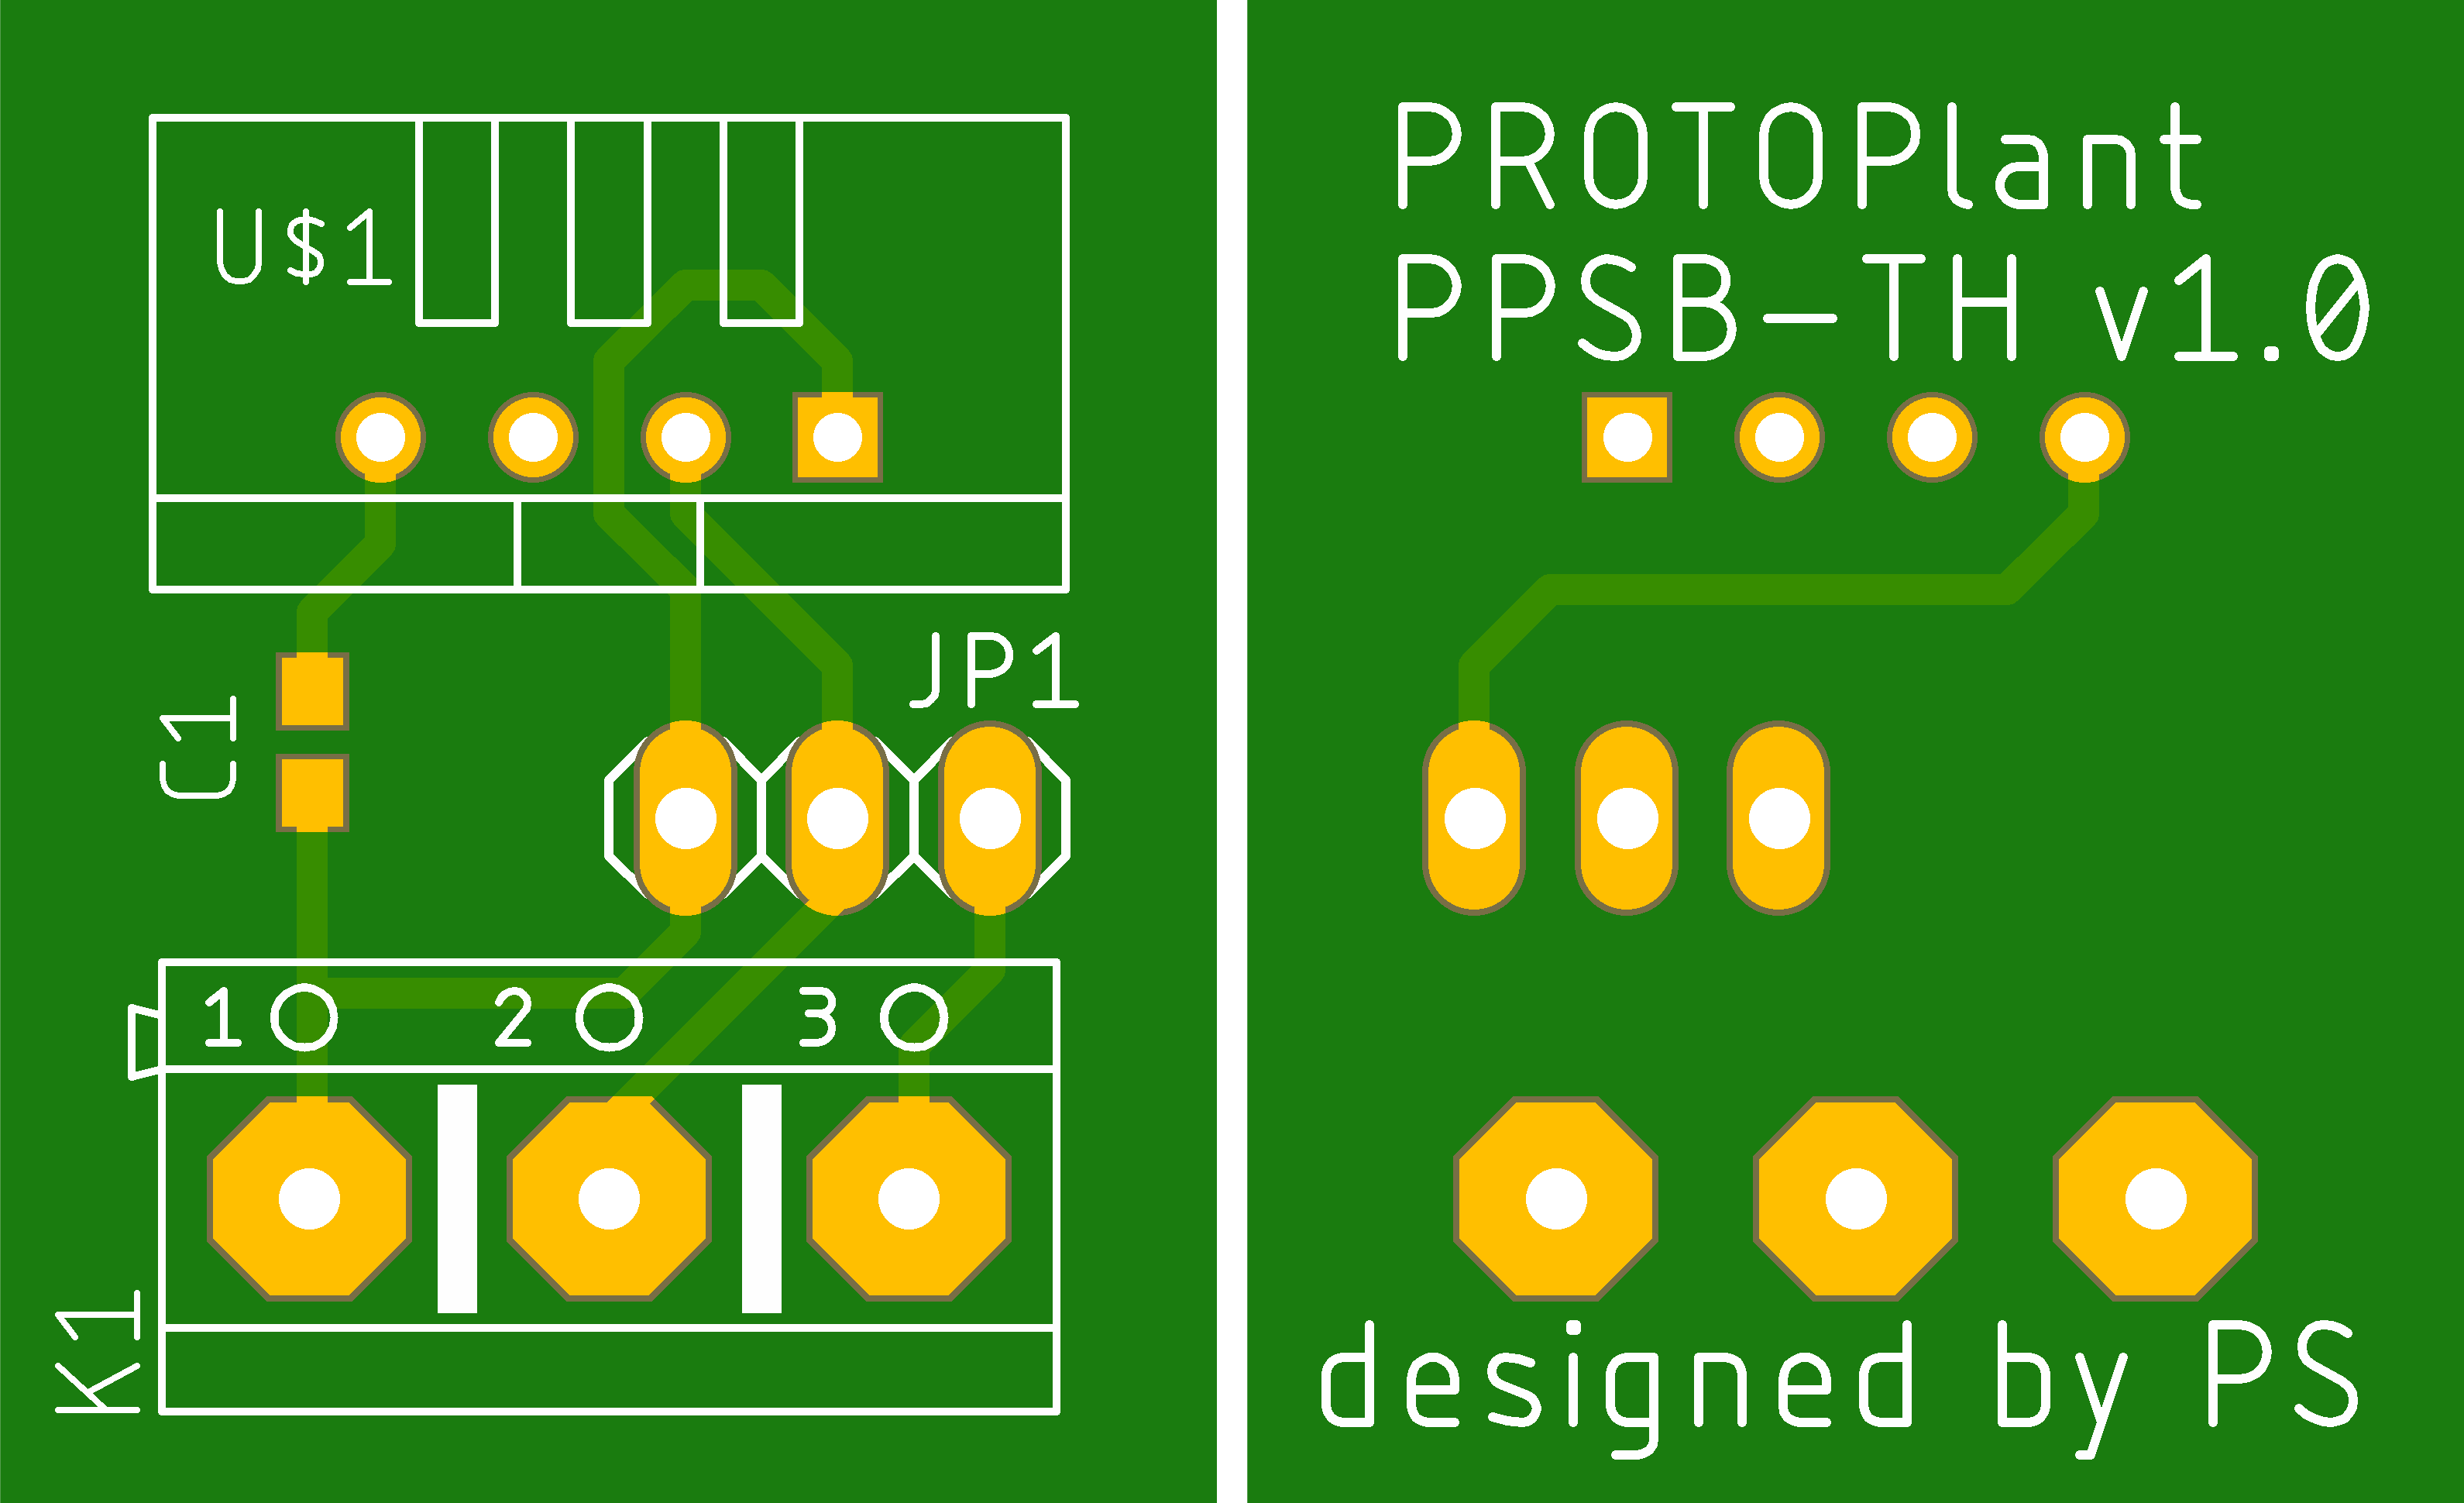
\includegraphics[width=0.85\textwidth]{img/HARDWARE/PPSB-TH_BOTH.png}
    \caption{Vizualizace desky PPSB-TH (horní strana vlevo, dolní vpravo).}
    \label{fig:PPSB-TH_VISUAL}
\end{figure}

\begin{figure}[htbp]
    \centering
    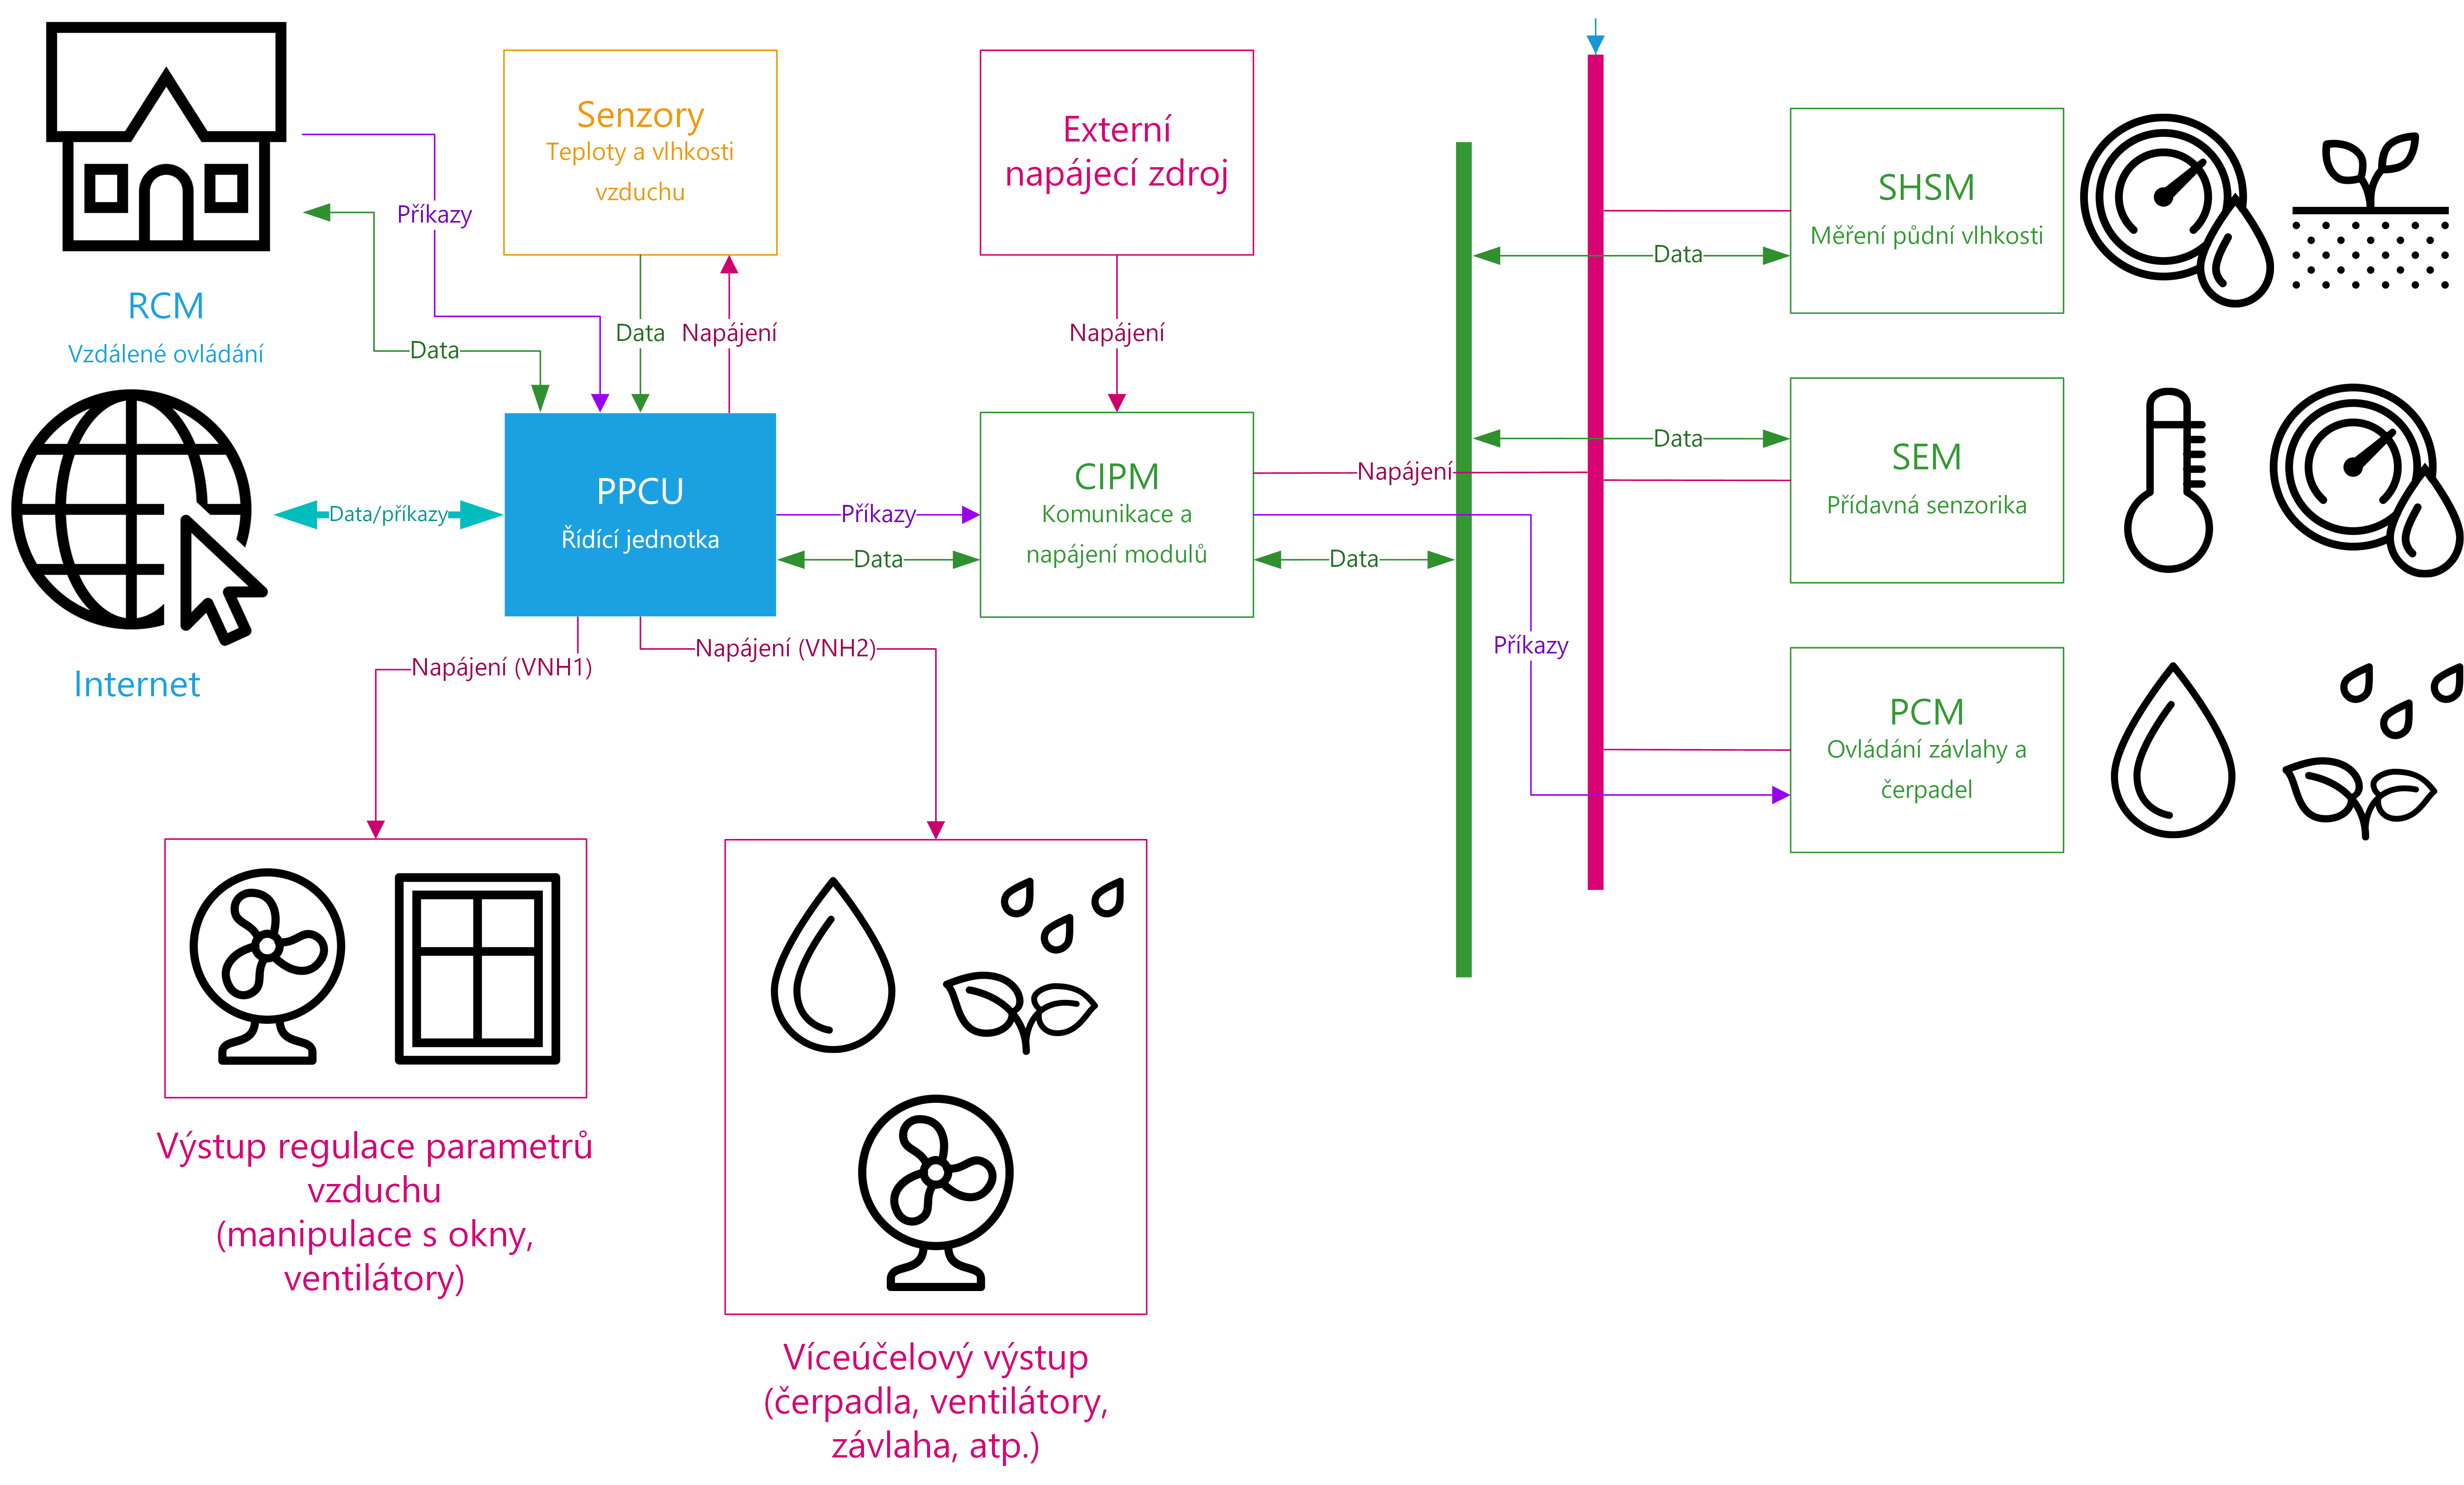
\includegraphics[angle=90,origin=c,scale=0.7]{img/HARDWARE/MODULES.png}
    \caption{Schéma zapojení a~funkce jednotlivých modulů.}
    \label{fig:add-MODULES}
 \end{figure}

\begin{figure}[h]
    \centering
    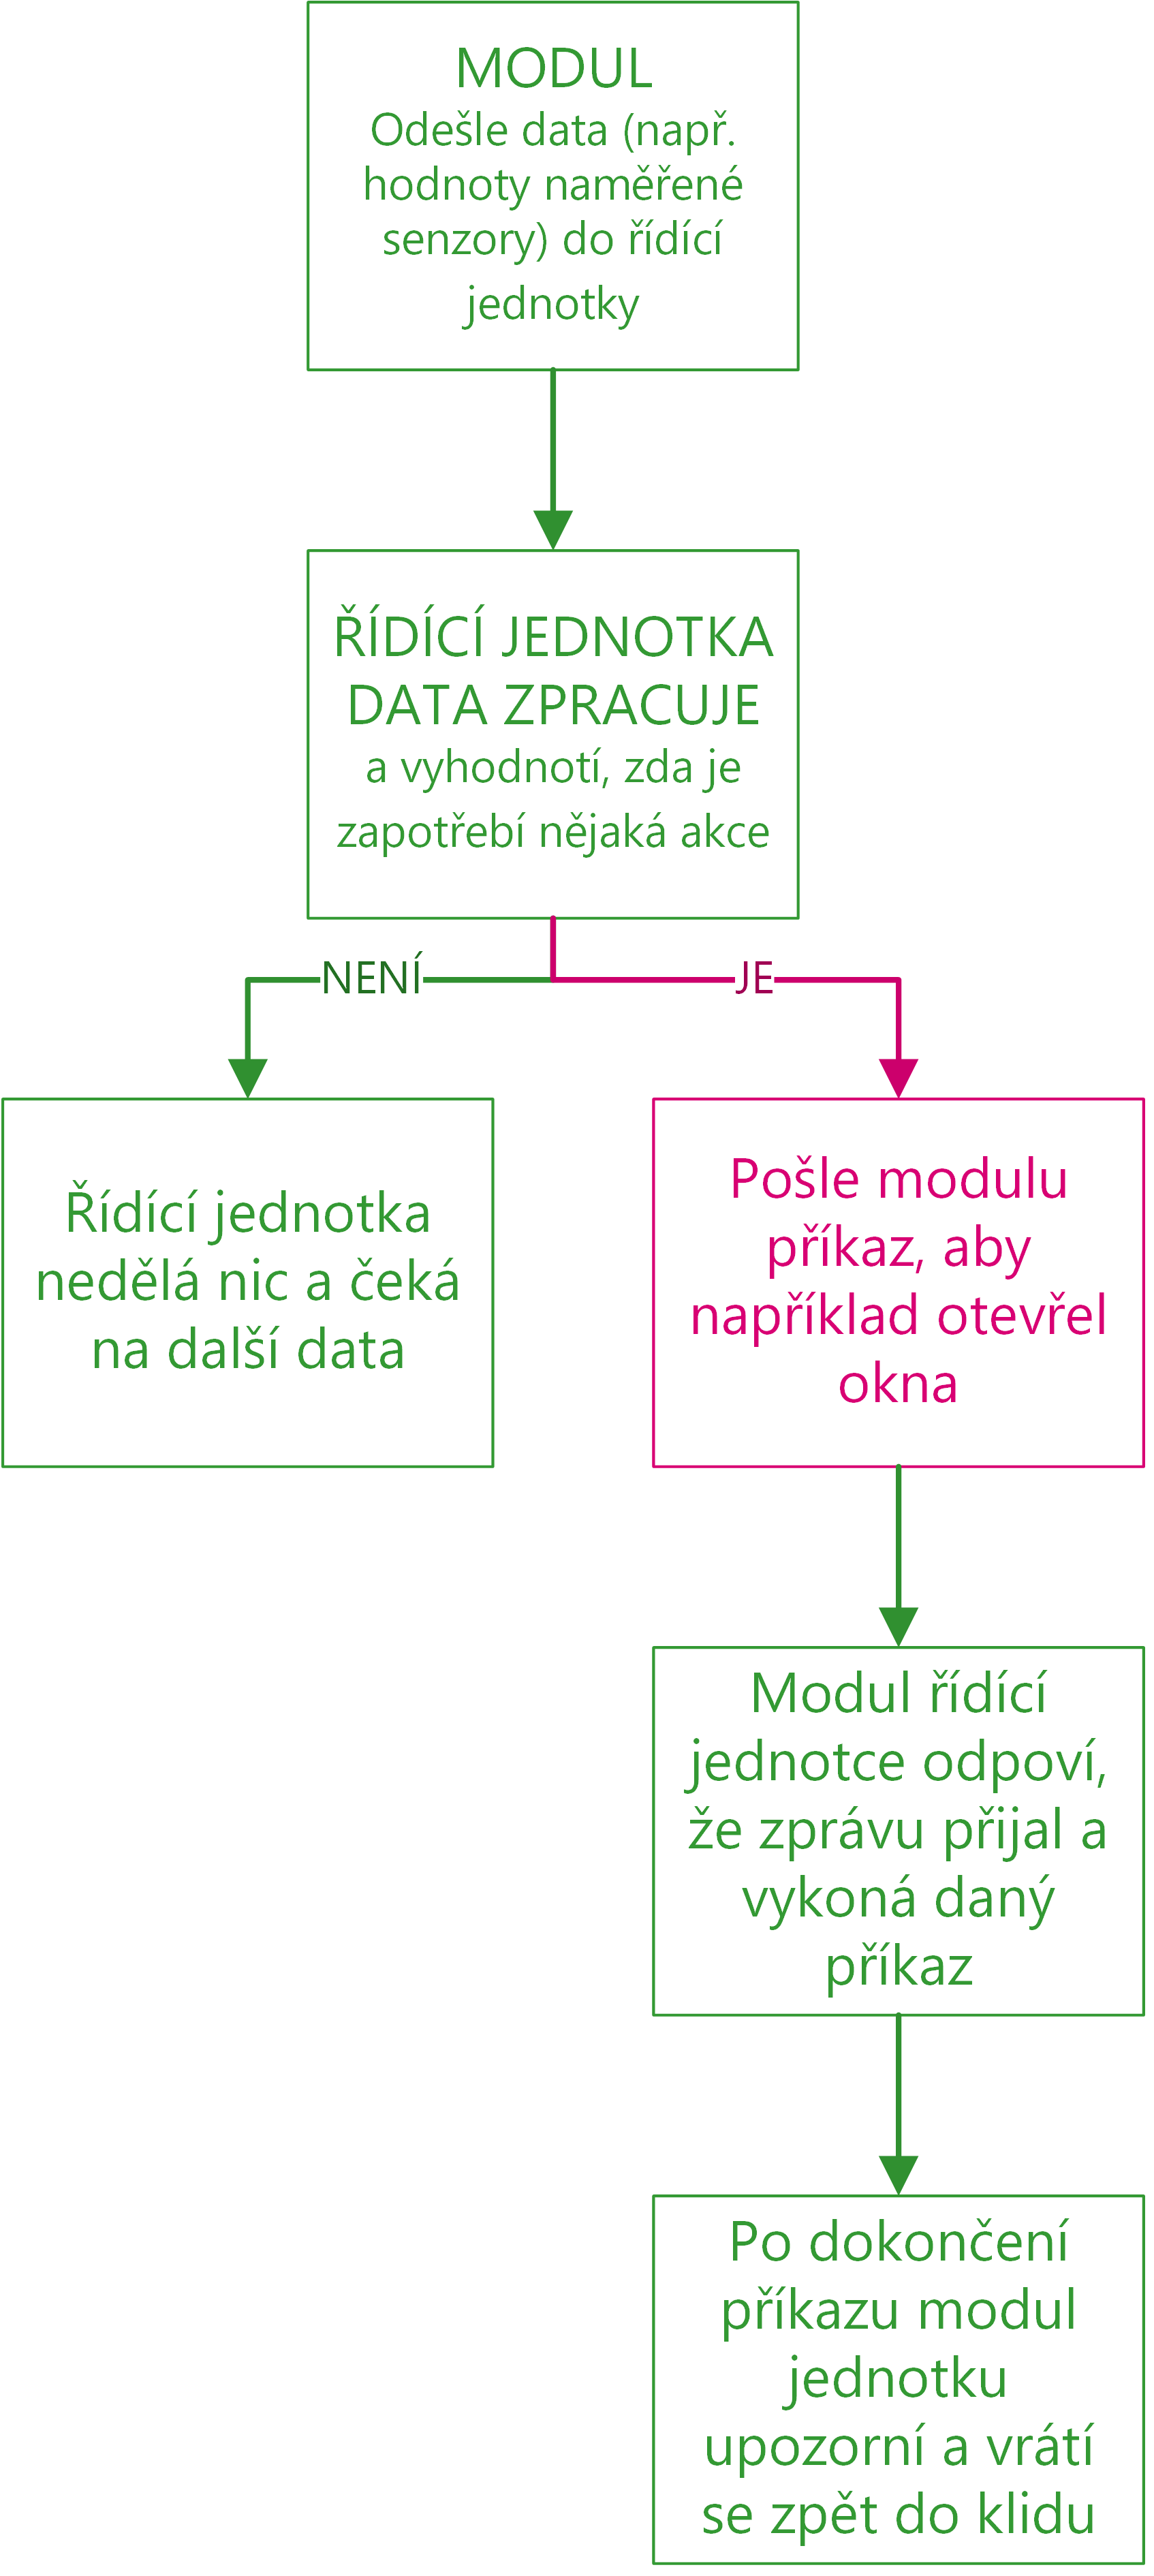
\includegraphics[scale=0.9]{img/SOFTWARE/KOMUNIKACE_MODULU.png}
    \caption{Blokový diagram komunikace řídící jednotky a~přídavného modulu.}
    \label{fig:PPCU-to-MODULE-communication}
\end{figure}

Stejným způsobem lze sázet další obrazové přílohy.
\newpage

\printbibliography[title=Literatura]
\addcontentsline{toc}{chapter}{Literatura}

\listoffigures
\addcontentsline{toc}{section}{Seznam obrázků}

\listoftables
\addcontentsline{toc}{section}{Seznam tabulek}

\end{document}
